\documentclass{article}
\usepackage{graphicx}
\usepackage{fitbox}
\begin{document}

We start from an image at maximal size:

{\centering\fitbox{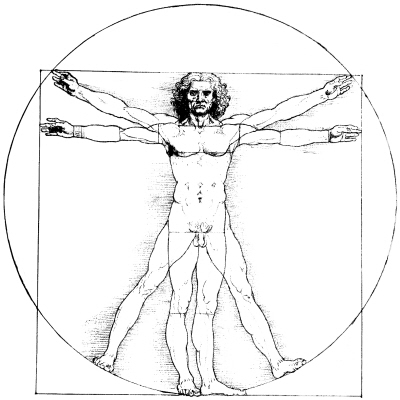
\includegraphics{vitruvian}}\par}

Now it is resized.  Here we allow down to 50\% of scale:

{\centering\fitbox[minheight=0.5\fitboxnatheight,
  minwidth=0.5\fitboxnatwidth]{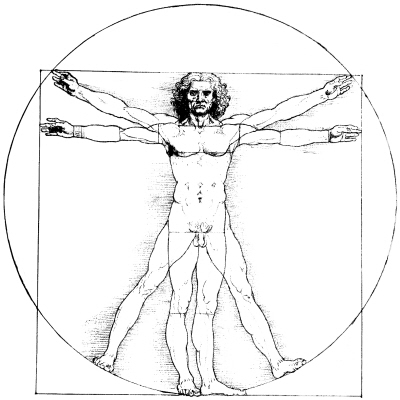
\includegraphics{vitruvian}}\par}




Now we make the figure smaller:

{\centering\fitbox[maxwidth=\fitboxnatwidth, 
  maxheight=\fitboxnatwidth]{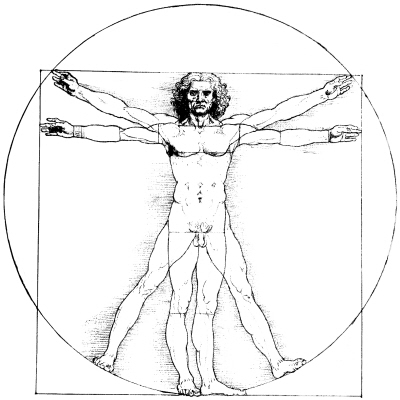
\includegraphics{vitruvian}}\par}

{\centering\fitbox[maxwidth=\fitboxnatwidth, 
  maxheight=\fitboxnatwidth]{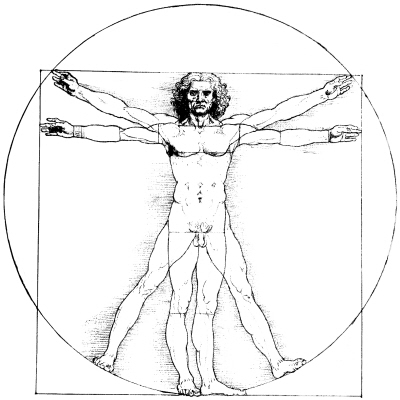
\includegraphics{vitruvian}}\par}



We leave some space, so the full size figure would not fit anymore:

{\centering\fitbox{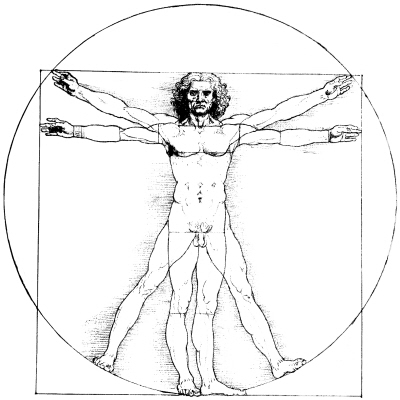
\includegraphics{vitruvian}}\par}

The figure is now on the next page.  Let us leave some space under the
next figure:

{\centering\fitbox[minheight=0.5\fitboxnatheight,
  minwidth=0.5\fitboxnatwidth, 
  belowboxspace=\baselineskip]{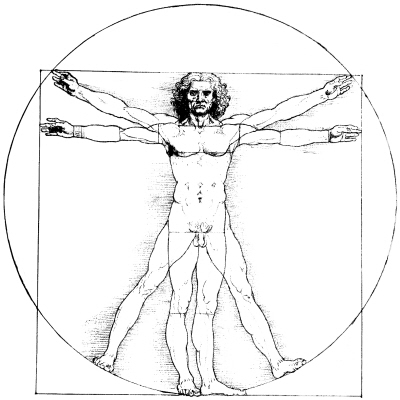
\includegraphics{vitruvian}}\par}
We left some space for a caption.

\end{document}
